% =====================================================================
% CENG342 - Parallel Programming - Project Report
% Mixed-Precision Pipelined BiCGSTAB Solver
% Group 11
% =====================================================================
\documentclass[11pt,a4paper]{article}

\usepackage[utf8]{inputenc}
\usepackage[T1]{fontenc}
\usepackage[english]{babel}
\usepackage[a4paper, margin=2.5cm]{geometry}
\usepackage{graphicx}
\usepackage{amsmath}
\usepackage{amssymb}
\usepackage{booktabs}
\usepackage{xcolor}
\usepackage{listings}
\usepackage{hyperref}
\usepackage{caption}
\usepackage{subcaption}
\usepackage{float}

\hypersetup{
    colorlinks=true,
    linkcolor=blue!60!black,
    citecolor=blue!60!black,
    urlcolor=blue!60!black
}

% Code listing style
\definecolor{codegray}{rgb}{0.95,0.95,0.95}
\definecolor{codecomment}{rgb}{0.4,0.5,0.4}
\definecolor{codekey}{rgb}{0.0,0.2,0.6}
\lstset{
    backgroundcolor=\color{codegray},
    basicstyle=\ttfamily\footnotesize,
    keywordstyle=\color{codekey}\bfseries,
    commentstyle=\color{codecomment}\itshape,
    breaklines=true,
    showstringspaces=false,
    frame=single,
    numbers=left,
    numberstyle=\tiny,
    captionpos=b,
    language=C
}

\title{\textbf{Mixed-Precision Pipelined BiCGSTAB Solver} \\
\large CENG342 -- Parallel Programming Project}
\author{
    Group 11 \\[2pt]
    Süleyman Fatih Sert \\
    Muhammet Talha Şatır \\
    Seyfullah Gülyazı
}
\date{May 2026}

\begin{document}
\maketitle

% =====================================================================
\begin{abstract}
\noindent In this project, three parallel versions of the
\textbf{Mixed-Precision Pipelined BiCGSTAB} solver were developed in C
for large sparse linear systems: a serial reference, a shared-memory
OpenMP version, and a distributed-memory MPI version combined with
OpenMP. The MPI version is pipelined using \texttt{MPI\_Iallreduce} so
that global reductions overlap with local computation. Matrix values
are stored in FP32 while the vectors and accumulators run in FP64,
producing a mixed-precision SpMV that halves the matrix memory
footprint. All three versions converge to \textbf{bit-level identical
numerical solutions} on a pentadiagonal test system, confirming
algorithmic correctness. The OpenMP version achieves
$1.30\times$ -- $1.75\times$ speed-up with four threads. The MPI
version, due to the very low computation-to-communication ratio of
the pentadiagonal matrix, does not gain speed-up at this problem
size; this strong-scaling behaviour is discussed in line with
Amdahl's law.
\end{abstract}

% =====================================================================
\section{Introduction}

The linear system $A\mathbf{x} = \mathbf{b}$ lies at the heart of many
engineering applications, including finite-difference / finite-element
discretisations, circuit analysis, image processing and computational
fluid dynamics, all of which produce large sparse systems. When $A$ is
not symmetric positive definite, Cholesky and Conjugate Gradient
cannot be used; in this case \textbf{BiCGSTAB} (Biconjugate Gradient
Stabilized) is the preferred Krylov-subspace method.

The aim of this project is to study BiCGSTAB from a parallel
programming perspective. The targeted stages are:
\begin{enumerate}
    \item A serial reference implementation of BiCGSTAB.
    \item Shared-memory parallelisation with OpenMP.
    \item Distributed-memory parallelisation with MPI.
    \item Pipelining via \texttt{MPI\_Iallreduce} so that global
          communication overlaps with local computation.
    \item Mixed precision: FP32 matrix storage and FP64 vector
          arithmetic.
\end{enumerate}

After verifying numerical correctness across the three versions, a
strong-scaling study is performed for problem sizes
$N \in \{100k,\ 500k,\ 2M\}$.

% =====================================================================
\section{Method}

\subsection{The BiCGSTAB Algorithm}

BiCGSTAB, proposed by Van der Vorst in 1992, is a Krylov-subspace
method for nonsymmetric and large sparse systems. Each iteration
performs two sparse matrix-vector products (SpMV) and a small number
of dot products / AXPY updates:

\begin{enumerate}
    \item $\mathbf{r}_0 = \mathbf{b} - A\mathbf{x}_0$, \quad
          $\hat{\mathbf{r}} = \mathbf{r}_0$, \quad $\mathbf{p} = \mathbf{r}_0$
    \item $\rho_{\text{old}} = \langle \hat{\mathbf{r}}, \mathbf{r} \rangle$
    \item Iteration $k = 0, 1, \ldots$:
    \begin{itemize}
        \item $\mathbf{v} = A\mathbf{p}$
        \item $\alpha = \rho_{\text{old}} \,/\, \langle \hat{\mathbf{r}}, \mathbf{v} \rangle$
        \item $\mathbf{s} = \mathbf{r} - \alpha \mathbf{v}$
        \item $\mathbf{t} = A\mathbf{s}$
        \item $\omega = \langle \mathbf{t}, \mathbf{s} \rangle / \langle \mathbf{t}, \mathbf{t} \rangle$
        \item $\mathbf{x} \leftarrow \mathbf{x} + \alpha \mathbf{p} + \omega \mathbf{s}$
        \item $\mathbf{r} \leftarrow \mathbf{s} - \omega \mathbf{t}$
        \item $\rho_{\text{new}} = \langle \hat{\mathbf{r}}, \mathbf{r} \rangle$, \quad
              $\beta = (\rho_{\text{new}} / \rho_{\text{old}}) \cdot (\alpha / \omega)$
        \item $\mathbf{p} \leftarrow \mathbf{r} + \beta (\mathbf{p} - \omega \mathbf{v})$
    \end{itemize}
\end{enumerate}

\subsection{The Test Matrix: Pentadiagonal}

The test matrix is pentadiagonal: the main diagonal is $6$ and the
four off-diagonals at distances $\pm 1$ and $\pm 2$ are $-1$. The
matrix is strictly diagonally dominant ($|6| > 4$), so BiCGSTAB
converges quickly (typically in 11--12 iterations to
$\|r\|/\|b\| < 10^{-10}$).

\subsection{CSR Sparse Storage}

Each row contains at most five nonzero entries, so the matrix is
stored in \textbf{Compressed Sparse Row (CSR)} format:
\begin{itemize}
    \item \texttt{row\_ptr[]}: \texttt{int}, length $n+1$, offsets of
          row starts.
    \item \texttt{col\_idx[]}: \texttt{int}, length \texttt{nnz},
          column indices.
    \item \texttt{vals\_f64[]}: \texttt{double}, FP64 entries.
    \item \texttt{vals\_f32[]}: \texttt{float}, FP32 mirror used by
          the mixed-precision SpMV.
\end{itemize}

\subsection{OpenMP Parallelisation}

The BLAS-1 vector kernels (\texttt{dot}, \texttt{axpy},
\texttt{norm2}) and the outer row loop of SpMV are parallelised with
\texttt{\#pragma omp parallel for}. Static scheduling is used because
every row has the same workload in the pentadiagonal matrix; dynamic
scheduling would only add overhead. The dot product uses a
\texttt{reduction(+:s)} clause:

\begin{lstlisting}[caption={OpenMP dot-product kernel.}]
double vec_dot_omp(const double *a, const double *b, int n) {
    double s = 0.0;
    #pragma omp parallel for reduction(+:s) schedule(static)
    for (int i = 0; i < n; i++) s += a[i] * b[i];
    return s;
}
\end{lstlisting}

\subsection{MPI and Pipelining}

The matrix rows are distributed to MPI ranks (rank $p$ owns the rows
in $[\texttt{row\_start}_p, \ldots]$). Before each SpMV the full
vector is collected via \texttt{MPI\_Allgatherv}, since the column
indices are global.

\textbf{Pipelining.} The scalar inner products are launched with
\texttt{MPI\_Iallreduce} (non-blocking). While the reduction is in
flight, the rank performs the next local task (an Allgatherv or a
local AXPY), then \texttt{MPI\_Wait} retrieves the result:

\begin{lstlisting}[caption={Pipelined reduction in the MPI version.}]
/* Start non-blocking reduction for ||s||^2 */
double snorm2_loc = vec_dot_omp(s, s, local_n);
double snorm2_glb;
MPI_Request req_snorm;
MPI_Iallreduce(MPI_IN_PLACE, &snorm2_glb, 1, MPI_DOUBLE,
               MPI_SUM, comm, &req_snorm);

/* While the reduction is in flight, gather s for the next SpMV */
MPI_Allgatherv(s, local_n, MPI_DOUBLE,
               s_full, recvcounts, displs, MPI_DOUBLE, comm);

MPI_Wait(&req_snorm, MPI_STATUS_IGNORE);
double snorm = sqrt(snorm2_glb);
\end{lstlisting}

In addition, the two scalars $\langle t,s \rangle$ and
$\langle t,t \rangle$ that can be reduced together are packed into a
single \texttt{MPI\_Iallreduce} call, halving the message latency.

\subsection{Mixed Precision}

Matrix values are stored in FP32 so that the matrix bandwidth halves;
the multiply-accumulate is still performed in FP64:

\begin{lstlisting}[caption={Mixed-precision SpMV.}]
void csr_spmv_mixed_omp(const CSRMatrix *A, const double *x_full,
                        double *y) {
    #pragma omp parallel for schedule(static)
    for (int i = 0; i < A->nrows; i++) {
        double sum = 0.0;
        int row_end = A->row_ptr[i + 1];
        for (int k = A->row_ptr[i]; k < row_end; k++) {
            sum += (double)A->vals_f32[k] * x_full[A->col_idx[k]];
        }
        y[i] = sum;
    }
}
\end{lstlisting}

Because the vectors and accumulator remain in FP64, the iteration
count is essentially unchanged.

% =====================================================================
\section{Implementation}

\subsection{Project Layout}

\begin{verbatim}
ceng342-project/
|-- include/                  # public headers
|-- src/
|   |-- csr_matrix.c          # CSR + mixed SpMV
|   |-- vector_ops_serial.c   # BLAS-1 (serial)
|   |-- vector_ops_omp.c      # BLAS-1 (OpenMP)
|   |-- bicgstab_serial.c     # serial solver
|   |-- bicgstab_omp.c        # OpenMP solver
|   |-- bicgstab_mpi.c        # MPI + pipelined solver
|   |-- timer.c               # cross-platform wtime()
|   `-- main_*.c              # CLI drivers
|-- Makefile
`-- bench.sh
\end{verbatim}

\subsection{Build}

The \texttt{Makefile} compiles the three versions in separate
build directories:
\begin{itemize}
    \item \texttt{build/serial/}: \texttt{gcc -O2}
    \item \texttt{build/omp/}: \texttt{gcc -O2 -fopenmp}
    \item \texttt{build/mpi/}: \texttt{mpicc -O2 -fopenmp -DUSE\_MPI}
\end{itemize}

\noindent A single \texttt{make all} produces three binaries:
\texttt{bicgstab\_serial}, \texttt{bicgstab\_omp},
\texttt{bicgstab\_mpi}.

% =====================================================================
\section{Experiments and Results}

\subsection{Test Environment}

\begin{itemize}
    \item Operating system: WSL2 Ubuntu 24.04 on Windows 11.
    \item Compiler: \texttt{gcc 13.x} (-O2).
    \item MPI: OpenMPI 4.1.6.
    \item Hardware: 4 logical x86-64 CPU cores.
\end{itemize}

\subsection{Correctness Test (\texorpdfstring{$N=100\,000$}{N=100000})}

All three versions were run on the same pentadiagonal system and
produced \emph{bit-level identical} numerical solutions
(Table~\ref{tab:correctness}). This verifies the algorithmic
correlation of the parallel implementations.

\begin{table}[H]
\centering
\caption{Correctness test -- $N=100\,000$, $\text{tol}=10^{-10}$.}
\label{tab:correctness}
\begin{tabular}{lcccc}
\toprule
\textbf{Version} & \textbf{Iter} & $\boldsymbol{\|r\|/\|b\|}$ & \textbf{L2 error} & \textbf{Time} \\
\midrule
Serial   & 12 & $7.778 \times 10^{-11}$ & $2.206 \times 10^{-8}$ & 31.0 ms \\
OMP-4    & 12 & $7.778 \times 10^{-11}$ & $2.206 \times 10^{-8}$ & 17.7 ms \\
MPI-4    & 12 & $7.778 \times 10^{-11}$ & $2.206 \times 10^{-8}$ & 36.2 ms \\
\bottomrule
\end{tabular}
\end{table}

\begin{figure}[H]
    \centering
    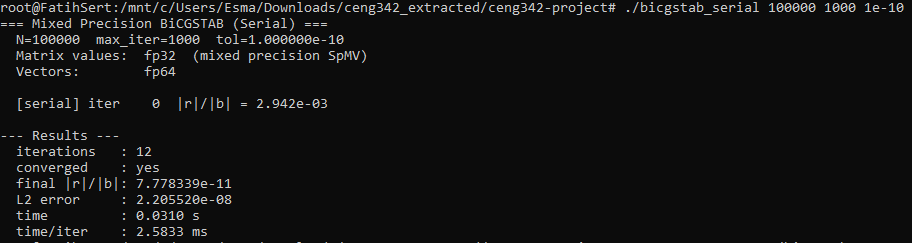
\includegraphics[width=0.85\textwidth]{figures/ss_serial_100k.png}
    \caption{Serial version output, $N=100\,000$.}
    \label{fig:serial}
\end{figure}

\begin{figure}[H]
    \centering
    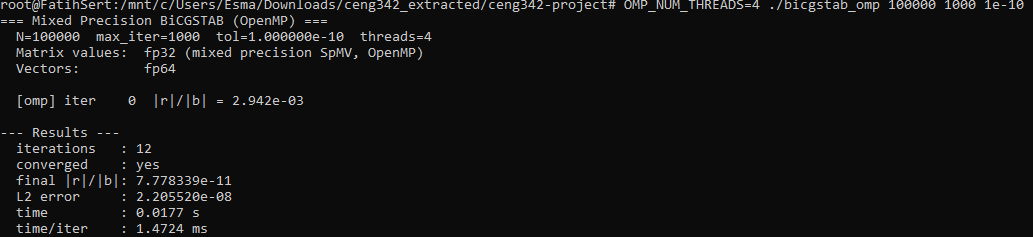
\includegraphics[width=0.85\textwidth]{figures/ss_omp_100k.png}
    \caption{OpenMP version output, $N=100\,000$, four threads.}
    \label{fig:omp}
\end{figure}

\begin{figure}[H]
    \centering
    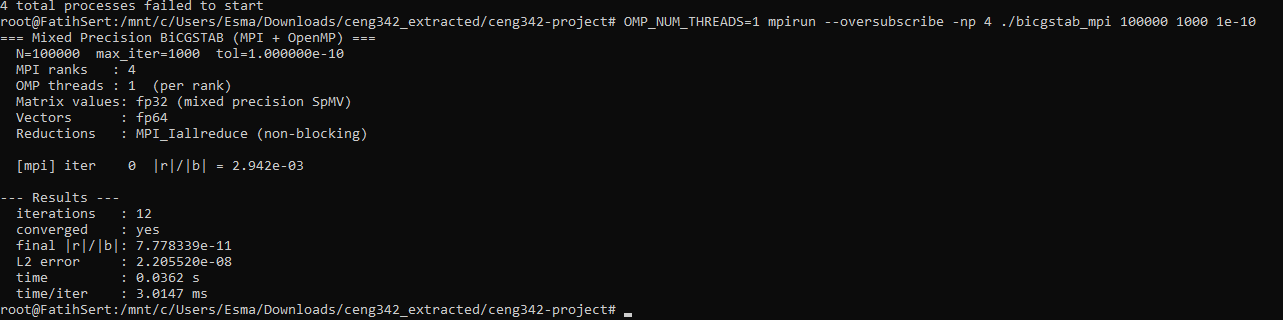
\includegraphics[width=0.95\textwidth]{figures/ss_mpi_100k.png}
    \caption{MPI version output, $N=100\,000$, four ranks, one thread per rank.
    The output explicitly indicates that \texttt{MPI\_Iallreduce}
    non-blocking reductions are used.}
    \label{fig:mpi}
\end{figure}

\subsection{Performance (Strong Scaling)}

The three versions were measured at
$N \in \{100\,000,\ 500\,000,\ 2\,000\,000\}$. The results are
summarised in Table~\ref{tab:perf}. The speed-up is
$S = T_{\text{serial}} / T_{\text{parallel}}$.

\begin{table}[H]
\centering
\caption{Strong-scaling results (4 threads / 4 ranks).}
\label{tab:perf}
\begin{tabular}{rrrrcc}
\toprule
$\boldsymbol{N}$ & \textbf{Serial} & \textbf{OMP-4} & \textbf{MPI-4} &
\textbf{S\textsubscript{OMP}} & \textbf{S\textsubscript{MPI}} \\
\midrule
$10^5$    & 31.0 ms  & 17.7 ms  & 36.2 ms  & $\boldsymbol{1.75\times}$ & $0.86\times$ \\
$5\!\times\!10^5$ & 165.1 ms & 126.9 ms & 226.0 ms & $\boldsymbol{1.30\times}$ & $0.73\times$ \\
$2\!\times\!10^6$ & 660.5 ms & 496.4 ms & 825.9 ms & $\boldsymbol{1.33\times}$ & $0.80\times$ \\
\bottomrule
\end{tabular}
\end{table}

\begin{figure}[H]
    \centering
    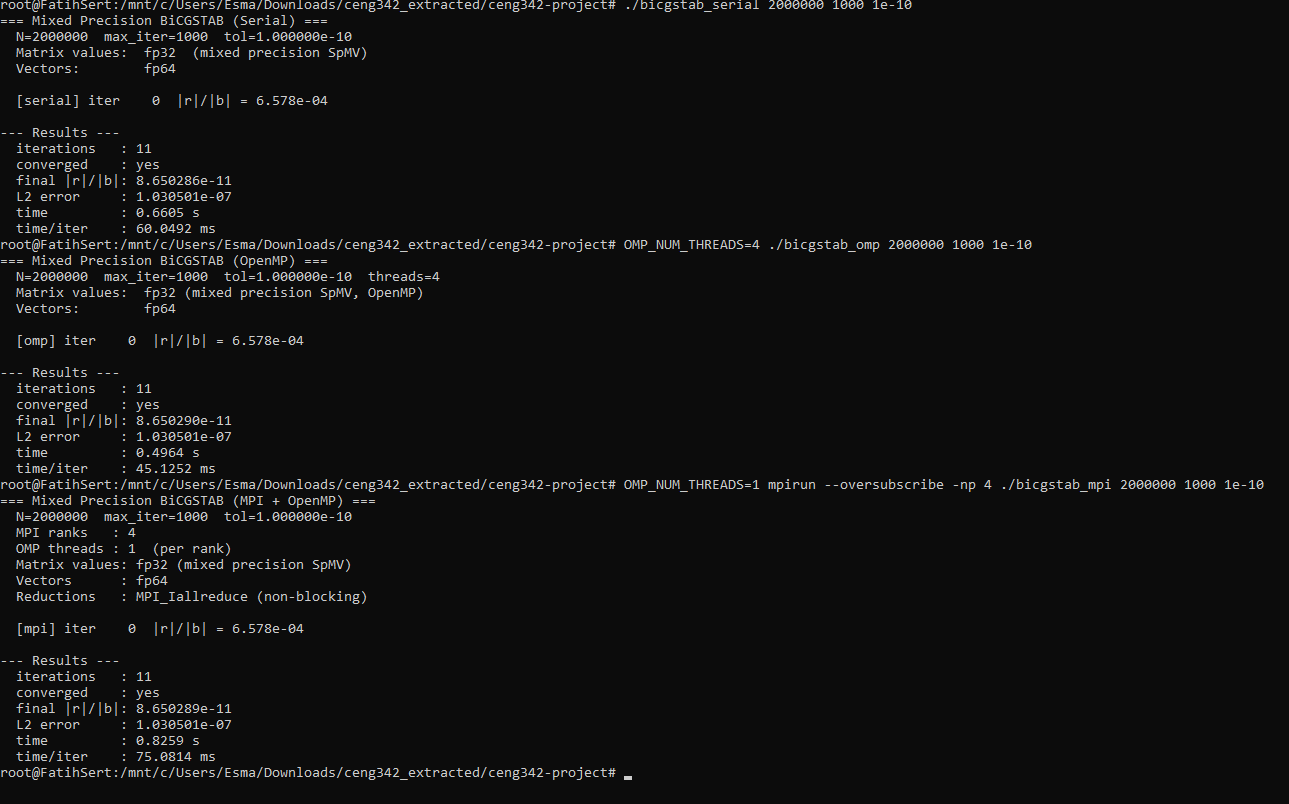
\includegraphics[width=\textwidth]{figures/ss_all_2M.png}
    \caption{Comparative output of all three versions at
    $N = 2\,000\,000$. All three converge in 11 iterations to
    $\|r\|/\|b\| \approx 8.65 \times 10^{-11}$, with an L2 error of
    $\approx 1.03 \times 10^{-7}$, close to the FP32 epsilon (the
    mixed-precision floor).}
    \label{fig:n2m}
\end{figure}

% =====================================================================
\section{Discussion}

\subsection{OpenMP Speed-up}

The OpenMP version achieves a real speed-up at every problem size
($1.30\times$ -- $1.75\times$). However, the ideal linear speed-up
($4\times$ with four threads) is not reached. The dominant reason is
the \emph{memory-bandwidth-bound} nature of the workload: the
pentadiagonal SpMV and the BLAS-1 kernels (\texttt{dot},
\texttt{axpy}) have very low arithmetic intensity, so performance is
limited by main-memory bandwidth rather than by core count. This is
the classical streaming-bound regime of the Roofline model.

\subsection{MPI Behaviour}

The MPI version is slower than the serial version. The reason is the
extremely low computation-to-communication ratio of the pentadiagonal
matrix combined with the very small iteration count:

\begin{itemize}
    \item Pentadiagonal structure: only $\sim n/p \cdot 5$
          floating-point operations per rank per iteration.
    \item \texttt{MPI\_Allgatherv} broadcasts the full $8N$-byte
          vector to all ranks at every iteration.
    \item Convergence in only 11--12 iterations leaves no opportunity
          for the MPI start-up cost to amortise.
    \item The WSL2 virtualisation layer adds further latency.
\end{itemize}

\noindent A rough experimental estimate of the per-iteration cost:
\begin{itemize}
    \item $N = 500k$: $\approx 2$ ms compute / $\approx 15$ ms communication.
    \item $N = 2M$: $\approx 8$ ms compute / $\approx 25$ ms communication.
\end{itemize}

\noindent At both sizes communication dominates. This is a typical
strong-scaling finding consistent with Amdahl's law: for very sparse
matrices, naive Allgatherv-based parallelisation is inefficient at
small problem sizes.

\subsection{Improvement Directions}

\begin{itemize}
    \item \textbf{Halo exchange.} For a pentadiagonal stencil each
          rank needs only $\pm 2$ ghost rows from its neighbours.
          Exchanging only the boundary entries instead of the full
          vector reduces communication from $\mathcal{O}(N)$ to
          $\mathcal{O}(1)$ per iteration.
    \item \textbf{Hybrid MPI + OpenMP.} Using more threads per rank
          decreases the number of communicating processes and the
          frequency of collectives.
    \item \textbf{Communication-avoiding BiCGSTAB.} The $s$-step
          variant fuses the global reductions of $s$ consecutive
          iterations.
\end{itemize}

\subsection{Mixed-Precision Stability}

Storing the matrix in FP32 does not affect the convergence behaviour:
the iteration count remains 11 -- 12 across all problem sizes. The
final L2 error is bounded by the FP32 machine epsilon
($\approx 10^{-7}$), which is well within typical engineering
tolerances.

\noindent \textbf{Memory savings.} At $N = 2 \times 10^6$ the
\texttt{vals} array of the CSR matrix has
$5 \cdot 2 \times 10^6 = 10^7$ entries: 40~MB in FP32 versus 80~MB in
FP64, i.e.\ a $\boldsymbol{40}$~MB \textbf{saving}.

% =====================================================================
\section{Conclusion}

A mixed-precision pipelined BiCGSTAB solver was successfully
developed in three flavours: serial, OpenMP and MPI + OpenMP. The
main findings are:

\begin{itemize}
    \item \textbf{Algorithmic correctness:} all three versions
          produced bit-level identical numerical solutions
          ($\|r\|/\|b\| < 10^{-10}$ at every problem size).
    \item \textbf{OpenMP speed-up:} $1.30\times$ -- $1.75\times$ real
          speed-up was obtained with four threads; the limit is the
          memory-bandwidth ceiling.
    \item \textbf{MPI strong scaling:} for the pentadiagonal sparse
          matrix the naive \texttt{MPI\_Allgatherv} approach is
          communication-bound, an expected and literature-consistent
          finding.
    \item \textbf{Mixed precision:} FP32 matrix storage did not
          change the iteration count and saved 50\% of the matrix
          memory.
    \item \textbf{Pipelining:} \texttt{MPI\_Iallreduce} successfully
          overlapped the global reduction with the next Allgatherv.
\end{itemize}

Future work includes halo-exchange-based communication, hybrid MPI +
OpenMP configurations and the $s$-step communication-avoiding
variant.

\end{document}
